\documentclass[../main.tex]{subfiles}
\begin{document}

\par In this chapter, I will conduct a literature review on the topic of predicting Acute Kidney Injury, especially in patients with Diabetic Ketoacidosis admitted to ICU.
The purpose of this chapter is to provide an overview of the current state of research on the topic, as well as to identify the gaps in the existing literature that this thesis aims to address.


\section{Scope of Research}
The scope of this chapter is centered on predicting AKI in patients with Diabetic Ketoacidosis  during their ICU admission, utilizing data from the MIMIC-IV database.
The emphasis lies on the development of novel predictive models and data engineering strategies tailored specifically for this population.
Thus, the focus will be on introducing innovative methodologies rather than extensively examining the relationships between AKI indicators or expanding the dataset.
In addition, the scope is limited current AKI definition by KDIGO guidelines \cite{kdigo-aki-guideline}, which is based on the changes in serum creatinine and urine output.


\section{Related Works}

Several studies have explored the prediction of Acute Kidney Injury in critical care settings, providing valuable insights into the development of predictive models and methodologies.

Firstly, the KDIGO guidelines \cite{kdigo-aki-guideline} offer standardized criteria for detecting AKI, serving as a foundational framework for AKI prediction studies.
The definition of AKI provided by KDIGO is based on the changes in serum creatinine and urine output, which are described as patients who satisfy at least one of the following criteria:

\begin{equation}
    \text{ Increase in SCr by } \geq 0.3 \text{ mg/dL } \text{ within 48 hours}
\end{equation}

\begin{equation}
    \text{ Increase in SCr to } \geq 1.5 \times \text{ baseline }
\end{equation}
The baseline is known or presumed to have occurred within the prior 7 days.

\begin{equation}
    \text{ Urine volume } \le 0.5 \text{ ml/kg/h for 6 hours}
\end{equation}

Although the KDIGO guidelines provide a standardized definition of AKI, upon detecting AKI, the damage has already occurred due to either high levels of creatinine or accumulation of waste products in the blood.
And the need for early prediction of AKI is demanding to prevent further complications and improve patient outcomes.
That is why my thesis aims to develop a predictive model that can detect the risk of AKI before the serious consequences occur.

While other studies struggled with the subtle nature of AKI, a study by \citeauthor{monogram-aki-dka} has developed a nomogram to predict the risk of Acute Kidney Injury for KDA-ICU patients.
This has shed light for the following researches as ICU patients got monitored more frequently than general patients, which could provide more accurate and abundant data for the prediction model.
On the flip side, the study used a deprecated definition of AKI and an older MIMIC version, leading falsely labeled AKI patients and small dataset.
Their best model, achieved an AUC of 0.747, which is a promising result but still has room for improvement.
One of my proposed upgrades is to use the latest MIMIC-IV database and the most recent definition of AKI to improve the model's accuracy.

Another study by \citeauthor{xgboost-aki-dka} has proposed using predictive models based on a machine learning approach to identify patients with DKA at increased risk of AKI within 1 week of hospitalization in the intensive care unit.
With state-of-the-art machine learning algorithms, the study achieved an AUC of 0.800, which is a significant improvement compared to the previous study.
However, the study did not take into account the changes in patients' indicators over time, which could be crucial for predicting Acute Kidney Injury as the disease progresses.
Moreover, the study did not provide a detailed process of extracting the features used in the model, making it difficult to replicate the results.
The researchers also use some features that are not available during real treatment process such as patient's lethality rate or continuous renal replacement therapy status of the patients which indicate the patient is already in serious stage of Acute Kidney Injury.
Thus, I planed to remove these features and add frequently occurring measurements as well as propose a new model that can consider the changes in patients' indicators.


% TODO: Add theoretical knowledge about models
\section{Predictive Models}


\subsection{Extreme Gradient Boosting (XGBoost)}

Proposed in \citetitle{xgboost-aki-dka}, XGBoost is currently state-of-the-art in machine learning algorithms for predicting AKI in patients with Diabetic Ketoacidosis.
The implication of XGBoost is reflected in the amount of studies that have utilized the algorithm to predict patient's outcomes like in \citetitle{other-xgboost-aki}, \citetitle{other-xgboost-mimic} or \citetitle{other-xgboost-mimic-2}.

Extreme Gradient Boosting (XGBoost) is an advanced implementation of the gradient boosting machine learning algorithm.
Developed by \citeauthor{xgboost-source} and the team at the University of Washington, XGBoost has gained immense popularity in the data science community due to its high performance and efficiency.
Gradient boosting is an ensemble learning technique that combines the predictions of several base learners to improve overall model performance.
XGBoost works as Newton approximation in function space unlike gradient boosting that works as gradient descent in function space, a second order Taylor approximation is used in the loss function to make the connection to Newton method.

For a given dataset, with n samples and m features, $\mathcal{D} = \{(x_1, y_1), (x_2, y_2), ..., (x_n, y_n)\}$, where $x_i \in \mathbb{R}^m$ is the feature vector and $y_i \in \mathbb{R}$ is the target value, XGBoost uses K additive functions to model the relationship between the features and the target variable:

\begin{equation}
    \hat{y_i} = \phi(x_i) = \sum_{k=1}^K f_k(x_i)
\end{equation}
in which, $f_k \in \mathcal{F}$ is a regression tree function, and $\mathcal{F}$ is the space of all possible regression trees.

\begin{figure}
    \centering
    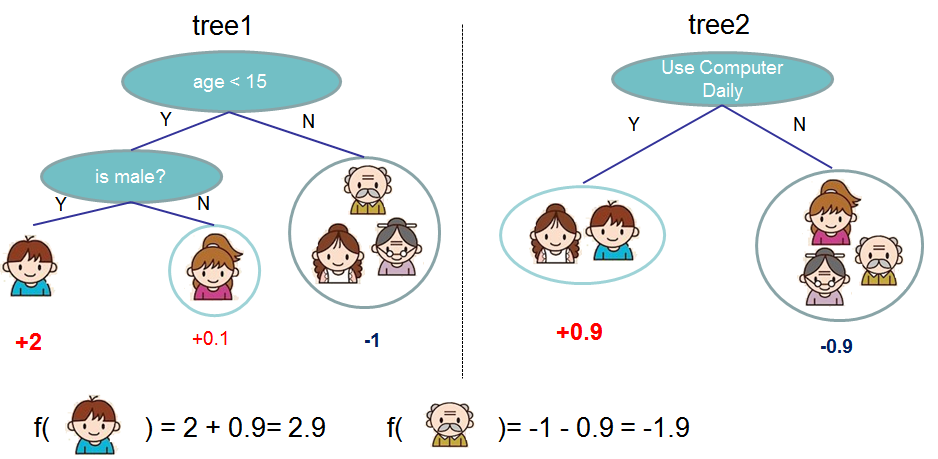
\includegraphics[width=.70\textwidth]{Figure/XGBoost_org_tree_model.png}
    \caption{Tree Ensemble Model. The final prediction for a given example is the sum of  predictions from each tree. By \citeauthor{xgboost-source}}
    \label{fig:treemodel}
\end{figure}


Each regression tree function $f_k$ is a binary tree structure that recursively partitions the feature space into disjoint regions, and assigns a constant value to each region.
Unlike traditional decision trees, the authors build regression trees to contain a continuous score in each leaf, rather than a discrete label.
$\omega_i$ is used to represent the leaf that the sample $x_i$ falls into.
Return to the example of the dataset $\mathcal{D}$, the prediction of the model is the sum of the leaf weights of the regression trees that the sample falls into.
To learn the set of functions used in model, the authors use the gradient boosting algorithm to optimize the loss objective:

\begin{equation}
    \begin{aligned}
        \mathcal{L}(\phi) =  \sum_{i=1}^n L(y_i, \hat{y_i}) + \sum_{k=1}^K \Omega(f_k) \\
        where \quad \Omega(f) = \gamma T + \frac{1}{2} \lambda ||w||^2
    \end{aligned}
\end{equation}

Here L is a differentiable convex loss function that measures the difference between the predicted value $\hat{y_i}$ and actual outcomes $y_i$;
$\Omega$ is the regularization term for model complexity (i.e., the regression tree functions), ensuring that the model does not overfit;
T is the number of leaves in the tree, and w is the leaf weights;
$\gamma$ and $\lambda$ are the regularization parameters that control the complexity of the model.

Let $\hat{y_i}^{(t)}$ be the prediction of the model at the t-th iteration, the authors update the model by adding a new regression tree function $f_t$ to minimize the loss function:

\begin{equation}
    \label{eq:added-loss}
    \begin{aligned}
        \mathcal{L}^{(t)} = \sum_{i=1}^n L(y_i, \hat{y_i}^{(t-1)} + f_t(x_i)) + \Omega(f_t) \\
        = \sum_{i=1}^n g_i f_t(x_i) + \frac{1}{2} h_i f_t^2(x_i) + \Omega(f_t)
    \end{aligned}
\end{equation}

where $g_i = \partial_{\hat{y_i}^{(t-1)}} L(y_i, \hat{y_i}^{(t-1)})$ and $h_i = \partial^2_{\hat{y_i}^{(t-1)}} L(y_i, \hat{y_i}^{(t-1)})$ are the first and second order gradients of the loss function, respectively.
After removing the constant terms, the authors can simplify the loss function to Eq.\ref{eq:added-loss}.

Expanding $\Omega$ and simplifying the loss function, the authors can derive the optimal leaf weights for the regression tree function $f_t$:

\begin{equation}
    \label{eq:optimal-leaf-weights}
    \begin{aligned}
        \hat{w}_{q} = - \frac{\sum_{i \in I_q} g_i}{\sum_{i \in I_q} h_i + \lambda}
    \end{aligned}
\end{equation}

Thus, the Eq.\ref{eq:added-loss} can be rewritten as:

\begin{equation}
    \begin{aligned}
        \mathcal{L}^{(t)}(q) = - \frac{1}{2} \sum_{i=1}^T \frac{(\sum_{i \in I_q} g_i)^2}{\sum_{i \in I_q} h_i + \lambda} + \gamma T
    \end{aligned}
\end{equation}

This equation is used to determine the quality of the tree $q$.
Since it is generally impossible to enumerate all possible trees, the authors use a greedy algorithm to find the optimal tree structure starting from a single leaf and recursively partitioning the feature space into disjoint regions.
With $I_L$ and $I_R$ are the left and right child nodes of the current node, the authors can calculate the loss reduction of the split:

\begin{equation}
    \begin{aligned}
        \mathcal{L}_{split} = \frac{1}{2} \left[ \frac{(\sum_{i \in I_L} g_i)^2}{\sum_{i \in I_L} h_i + \lambda} + \frac{(\sum_{i \in I_R} g_i)^2}{\sum_{i \in I_R} h_i + \lambda} - \frac{(\sum_{i \in I} g_i)^2}{\sum_{i \in I} h_i + \lambda} \right] - \gamma
    \end{aligned}
\end{equation}

Furthermore, the authors use 2 additional technique to prevent overfitting.
The first one is shrinkage which is a regularization technique that reduces the contribution of each tree by a factor $\eta$ after each iteration.
Similar to the learning rate in gradient descent, the shrinkage parameter $\eta$ reduce the influence of each tree on the final prediction, leaving more room for the model to learn from the data.
The second technique is features subsampling, which randomly selects a subset of features to split at each node, reducing the correlation between trees and improving the model's generalization ability and speed.

Another problem that \citeauthor{xgboost-source} tackled in their research is proposing candidate split points for each feature.
For tree-based models like XGBoost, it is important to find the optimal split points for each feature to maximize the loss reduction.
By defining the rank function as
\begin{equation}
    \label{eq:rank-function}
    \begin{aligned}
        r_k(z) = \frac{1}{\sum_{(x, h) \in \mathcal{D}_k}h} \sum_{(x, h) \in \mathcal{D}_k} h,
    \end{aligned}
\end{equation}
which represent the ratio of instances whose feature value is less than z in the dataset $\mathcal{D}_k$.
With this, the model can find candidate split points satisfying the condition:

\begin{equation}
    \begin{aligned}
        \lvert r_k (s_{k, j}) & - r_k (s_{k, j + 1}) \rvert < \epsilon \\
        s_{k1}                & = \min_{i} x_{ik}                      \\
        s_{kl}                & = \max_{i} x_{ik}
    \end{aligned}
\end{equation}

In this place, $\epsilon$ is an approximate factor which is roughly equal 1 \slash Number of candidate points.
If we rewrite Eq.\ref{eq:added-loss} as:

\begin{equation}
    \begin{aligned}
        \sum_{i=1}^{n} \frac{1}{2} h_i (f_t (x_i) - \frac{g_i}{h_i})^2 + \Omega(f_t) + Constant,
    \end{aligned}
\end{equation}

it can be clearly seen that this is weighted squared loss with labels $g_i$ \slash $h_i$ and weights $h_i$. So, $h_i$ is the weight of each data point in the loss function Eq.\ref{eq:rank-function}.

Another strength of XGBoost is its ability to handle missing values in the dataset or Sparsity-aware Split Finding.
In medical datasets, missing values are common due to the nature of the data collection process.
Many measurements are not taken regularly due to not being crucial for certain patients in certain period of hospitalization or the limitation of hospitalization facilities, leading to missing values in the dataset.
Thus, the ability to handle missing values automatically is a significant advantage of XGBoost making it appealing to medical researches.
When a value is missing, it is classified to default direction in the tree, and the algorithm will find the optimal split point for the missing values based on train data.
The authors even took a step further using the missing value to the model's advantage to make computational workload linear to the number of missing values.
This make XGBoost 50 times faster \cite{xgboost-source}.


\subsection{TabPFN}

Founded in \citetitle{tabpfn}, TabPFN has been proven to have a significant improvement in performance compared to traditional Gradient Boosting algorithms.
It was build on the foundation of Prior-Data Fitted Networks so the name is TabPFN.
PFNs approximate Posterior Predictive Distribution directly for Supervised Learning, which is a Bayesian approach to predictive modeling.

\textbf{The Posterior Predictive Distribution for Supervised Learning} \\
Defining a space of hypotheses $\Phi$ on the relationship of a set of inputs $x$ to the output label $y$.
Each hypothesis $\phi \in \Phi$ is a function generating a data distribution from which the authors draw samples forming a dataset.
Explained by \citeauthor{tabpfn}, given a prior based on structural causal models, $\Phi$ is the space of structural causal models, a hypothesis $\phi$ is one specific SCM, and a dataset comprises samples generated through this SCM.
In practice, a dataset comprises training data with observed labels and test data where labels are missing or held out to assess predictive performance.
The PPD for a test sample $x_{test}$ specifies the distribution of its label $p(\cdot|x_{test},D_{train})$, which is conditioned on the set of training samples $D_{train} := \{(x_1,y_1), \dots, (x_n,y_n)\}$.
The PPD can be obtained by integration over the space of hypotheses $\Phi$, where the weight of a hypothesis $\phi\in\Phi$ is determined by its prior probability $p(\phi)$ and the likelihood $p(D|\phi)$ of the data $D$ given $\phi$:
\begin{equation}
    p(y|x,D) \propto \int_{\Phi} p(y|x,\phi) p(D|\phi) p(\phi) d\phi.
    \label{eq:ppd}
\end{equation}


\textbf{Synthetic Prior-fitting}\\
Prior-fitting is a technique to approximate the PPD by fitting a parametric model to the posterior distribution of the hypothesis space.
In \citetitle{tabpfn}, it is implemented with a prior specified by sampling scheme of the form $p(D)=E_{\phi \sim p(\phi)}[p(D|\phi)]$, which start by sampling hypotheses with $\phi \sim p(\phi)$ and then synthesis data with the hypothesis $D \sim p(D|\phi)$.
Such synthesis datasets $D := (x_i, y_i)_{i \in \{1, \dots, n\}}$ are repeatedly resampled while parameters $\theta$ of PFN are optimized to predict $D_{test} \subset D$ | $D_{train} := D \setminus D_{test}$.
The loss function is defined as the negative log-likelihood of the test data:

\begin{equation}
    \mathcal{L}_{\textit{PFN}} = E_{(\{(x_{test}, y_{test})\} \cup D_{train}) \sim p(D)} [-\log q_{\theta}(y_{test}|x_{test},D_{train})].
    \label{eq:lpfn}
\end{equation}

\begin{figure}
    \begin{subfigure}{.5\textwidth}
        \centering
        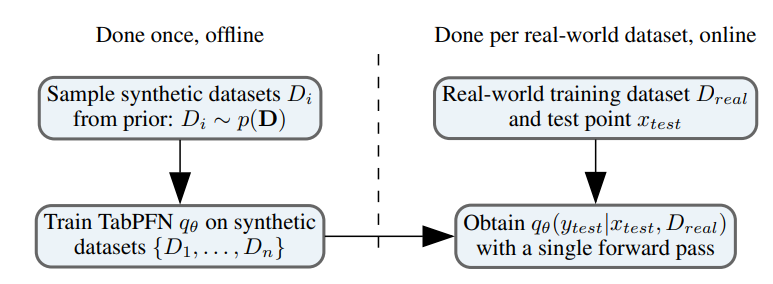
\includegraphics[width=.8\linewidth]{Figure/tabpfn_prior-fitting.png}
        \caption{Prior-fitting and inference}
        \label{fig:pfn_usage}
    \end{subfigure}
    \begin{subfigure}{.5\textwidth}
        \centering
        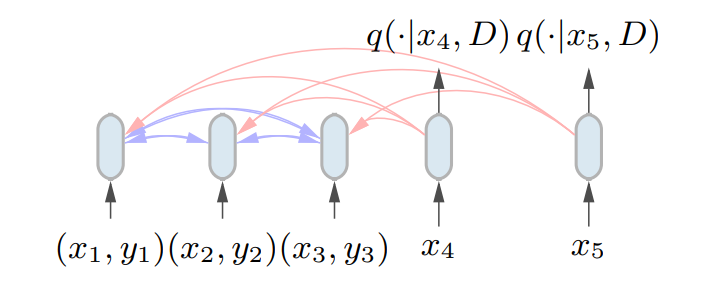
\includegraphics[width=.8\linewidth]{Figure/tabpfn_baysian_nodes.png}
        \caption{Architecture and attention mechanism}
        \label{fig:transformer_visualization}
    \end{subfigure}
    \caption{Left (a): The PFN learns to approximate the PPD of a given prior in the offline stage to yield predictions on a new dataset in a single forward pass in the online stage. Right (b): Training samples $\{(x_1,y_1), \dots, (x_3,y_3)\}$ are transformed to $3$ tokens, which attend to each other; test samples $x_4$ and $x_5$ attend only to the training samples. By \citeauthor{tabpfn}}
    \label{fig:pfn_overview}
\end{figure}

The backend of TabPFN can be condensed in the image \ref{fig:pfn_overview}.
Where the trained model is applied to unseen real-world datasets.
For a novel dataset with training samples $D_{train}$ and test features $x_{test}$, feeding $\langle{}D_{train},x_{test}\rangle$ as an input to the model trained above yields the PPD $q_{\theta}(y|x_{test},D_{train})$ in a single forward-pass.
The PPD class probabilities are then used as predictions for our real-world task.
Thus, PFNs perform training and prediction in one step (similar to prediction with Gaussian Processes) and do not use gradient-based learning on data seen at inference time.
This is in contrast to traditional neural networks, which require multiple forward and backward passes for training and prediction.


\section{Literature Conclusions}

In summary, this chapter has provided an overview of the existing literature on predicting Acute Kidney Injury (AKI) in patients with Diabetic Ketoacidosis (DKA) admitted to the Intensive Care Unit (ICU). The review covered the scope of research, key related works, and the potential of advanced predictive models like Extreme Gradient Boosting (XGBoost) and TabPFN in addressing this critical healthcare challenge.

The scope of the research is confined to utilizing data from the MIMIC-IV database and adhering to the KDIGO guidelines for AKI definition. This focus ensures the relevance and accuracy of the predictive models being developed. While KDIGO guidelines offer a standardized framework for AKI detection, the necessity for early prediction before severe consequences occur underscores the importance of developing more precise and timely models.

Related studies have highlighted the progression in predictive model accuracy and methodology. For instance, \citeauthor{monogram-aki-dka}'s study using nomograms and the XGBoost model proposed by \citeauthor{xgboost-aki-dka} have provided valuable insights and promising results, albeit with limitations that this thesis aims to address. The use of the latest MIMIC-IV database and a more refined approach to feature selection and temporal changes in patient indicators are among the enhancements proposed.

The chapter also delved into the theoretical foundations and practical implications of advanced predictive models. XGBoost, with its high performance and efficiency, and TabPFN, with its innovative approach to approximating Posterior Predictive Distributions, represent the cutting-edge techniques in this field. These models not only improve predictive accuracy but also offer robustness in handling complex, real-world medical datasets, including those with missing values.

By building on these foundations and addressing the identified gaps, this thesis aims to contribute to the development of more effective and reliable predictive models for AKI in DKA patients. The next chapter will delve into the methodology employed in this research, detailing the data preparation, feature engineering, model training, and evaluation processes that underpin the proposed predictive framework.

\end{document}